\section{Einführung}

	Das Jahr 1969 gilt heute als Geburtsstunde des Internets. Mithilfe des Telnet-Protokolls kommunizierten vier Rechner in Kalifornien und Utah miteinander und legten somit den Grundstein für eine Technologie, die die Welt im Laufe der Zeit veränderte wie kaum eine vor ihr. \cite{lmzgeschichte} Nur fünf Jahre später entwickeln Robert Kahn und Vinton Cerf gemeinsam das \ac{tcp} und machen damit erste Schritte hin zu einem modernen Netzwerk wie wir es heute kennen und nutzen.\\
	Als das \ac{www} 1990 am CERN in Genf entwickelt wird, handelt es sich noch um eine Kommunikationsplattform für Wissenschaftler. Zu diesem Zeitpunkt ist kaum zu erahnen, welche Trends sich im Jahr 2019 - nur ein halbes Jahrhundert nach dem Beginn des Internets - entwickeln. Die grundlegende Idee besteht heutzutage daraus, möglichst viele Geräte verschwindend geringer Größe an das Internet anzubinden, sodass sogar einzelne Sensoren selbstständig Daten an zentrale Server schicken können. Dieser technologische Wandel stellt Ingenieure und Informatiker vor ganz neue Herausforderungen, die es zu bewältigen gilt. \\
	Auf den ersten Blick ist nicht ganz ersichtlich, warum kleine Geräte schwieriger ins Internet zu integrieren sind als große. Die Problematik, dass das \ac{ipv4} durch die 32-bit \ac{ip}-Adresse nur $2^32\approx4.200.000.000$ verschiedene Teilnehmer adressieren kann ist durch das \ac{ipv6} und die Adressgröße von 128bit gelöst. Theoretisch böten die $2^128\approx$ 340 Sextillionen verschiedenen Adressen ausreichend Möglichkeiten, jedem denkbaren Gerät eine eigene \ac{ip}-Adresse zuzuordnen.\\
	Viel mehr sind es Probleme des lokalen Teilnehmers als des Netzwerks, die neue Technologien unabdingbar machen. Sowohl software- als auch hardwareseitig sind kleine Sensoren nämlich herkömmlich nicht dazu ausgelegt, internetfähig zu kommunizieren. Klassische \ac{ip}-Stacks überforderten in der Vergangenheit die Rechenleistung der - nicht selten 8-bit - Mikrocontroller, leistungshungrige Wi-Fi-Module arbeiten zu ineffizient für die meist durch kleine Knopfzellen angetriebenen Geräte. Kabelbasierte Kommunikation fällt aufgrund der flexiblen Anbringung von Sensoren als Lösung ohnehin meist aus. Diese Gründe sorgten dafür, dass die Teilnahme kleiner, leistungsschwacher, batteriebetriebener Geräte in der Vergangenheit unmöglich erschien. Heute gilt es als erreichbares Ziel und wird mit dem Schlagbegriff Internet der Dinge oder englisch \ac{iot} gekennzeichnet.\\
	Ein erster Schritt hin zu Realisierung dieses Ziels war der uIP-Stack. Als Adam Dunkels vom \ac{sics} ihn entwickelte, war er der erste IP-Stack, der kompiliert so klein war, dass er die geringe Speichermöglichkeit von Mikrocontrollern nicht überlastete. Abhängig vom eingesetzten C Compiler kann die Größe des kompilierten Stacks zwischen mehreren hundert Bytes bis hin zu wenigen Kilobytes betragen. Um den Speicherverbrauch des Stacks (Hinweis: Hier 'Stack' im Sinne von Speicher) möglichst gering zu halten, setzt uIP auf globale Variablen, um Werte zwischen Funktionen zu kommunizieren.\cite[S.5]{dunkelsuip} Das 2003 ebenfalls von Adam Dunkels entwickelte Betriebssystem Contiki, das in späteren Kapiteln besprochen wird, setzt auf diesem Stack auf.\\
	Dieses Dokument präsentiert ein Projekt, das auf Basis von Contiki ein \ac{6lowpan}-Netzwerk aufbaut. Dabei wird zunächst die Notwendigkeit des Protokolls \ac{6lowpan} und der darunter fallenden Norm \ac{15.4} - auch in Hinsicht ihres Beitrags zum Internet der Dinge - besprochen. Darauf folgend werden sukzessive die technischen Hintergründe von \ac{15.4}, \ac{6lowpan} und IPv6/UDP im Hinblick auf die Besonderheiten bzgl. \ac{6lowpan} erläutert. Dies soll eine Einführung in diese Technologie von Physical Layer bis hin zum Transport Layer des \ac{osi}-Modells darstellen. Daraufhin wird, um eine Realisierung eines Netzwerks auf Basis dieser Technik zu ermöglichen, eine Einführung in Contiki gegeben und zum Abschluss das konkrete Projekt erklärt. 

\subsection{Motivation}

Der Wunsch, kleine Geräte internetfähig zu machen, wurde bereits in der Einleitung erläutert. Um dieses Ziel zu erreichen, ist die Implementierung einer Reihe von Protokollen nötig.
\begin{figure}
	\centering
	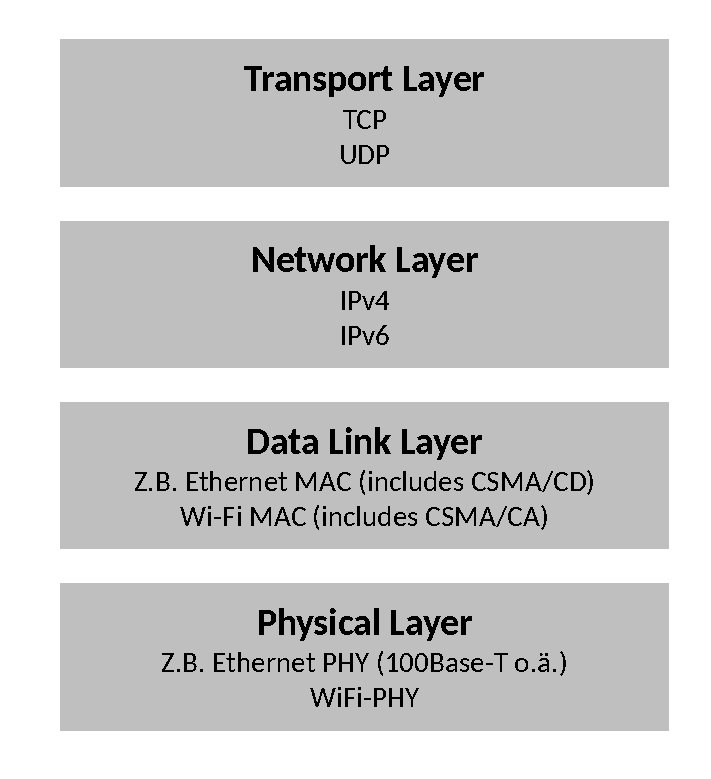
\includegraphics[width=\textwidth/2]{Grafiken-Alex/internet-osi.pdf}
	\caption{Beispielhafter Aufbau der ersten vier Schichten des \ac{osi}-Modells eines internetfähigen Geräts}
	\label{internet-osi}
\end{figure}
\begin{itemize}
	\item Layer 1 und 2 des \ac{osi}-Modells werden für gewöhnlich durch Techniken nach IEEE 802.11 (Wi-Fi) oder IEEE 802.3 (Ethernet) realisiert. Diese Normen sind nicht zwingend notwendig, um als Teilnehmer im Internet aufzutreten, sind aber gängige Lösungen.
	\item Zentraler Bestandteil des Internets ist \ac{ip} auf Layer 3. Erst durch dessen Implementierung kann ein Gerät am Internet teilnehmen.
	\item Auf Layer 4 sind die Protokolle \ac{udp} und \ac{tcp} gängig, um verbindungslos (\ac{udp}) oder verbindungsorientiert (\ac{tcp}) Daten zu verschicken.
\end{itemize}
Somit ergibt sich ein Aufbau der ersten vier Schichten des \ac{osi}-Modells wie in Grafik \ref{internet-osi}. 

Will man nun - wie es im \ac{iot} häufig der Fall ist - von einem Sensor Daten zur Verwaltung an einen zentralen Server schicken, so ist der Einsatz von \ac{udp} sinnvoll. Es handelt sich ohnehin meist um kleine Datensätze, die die Größe eines einzelnen \ac{ip}-Pakets nicht selten nicht überschreiten. Ein komplexer Verbindungsaufbau wie bei \ac{tcp} ist hierzu nicht nötig. Ein unterwegs verloren gegangenes Paket richtet durch die ständige Aktualisierung von Sensordaten kaum großen Schaden an.\\
Auf Layer 3 ist der Einsatz von \ac{ip} obligatorisch. Weil es sich bei \ac{ipv4} um ein veraltetes Protokoll handelt, das immer mehr von \ac{ipv6} verdrängt wird und moderne, zukunftsfähige Sensornetzwerke kaum noch darauf setzen, wird in dieser Ausarbeitung nur \ac{ipv6} betrachtet.\\
Bei den beiden unteren Layern ist der Einsatz kabelgebundener Lösungen kaum realistisch. Sensoren sollen die Möglichkeit bieten, ohne großen Montageaufwand flexibel eingesetzt werden zu können. Durch den geringen Stromverbrauch reichen schon einfache Knopfzellenbatterien als Energielieferant, weshalb eine Verlegung von Kabeln nur zu Kommunikationszwecken nicht sinnvoll wäre. Lösungen wie Ethernet fallen somit weg und auf den ersten Blick erscheint der Einsatz von Wi-Fi sinnvoll. Somit ergäbe sich ein tatsächlicher Aufbau der ersten vier Schichten des \ac{osi}-Modells wie in Grafik \ref{sensor-osi} gezeigt.
\begin{figure}
	\centering
	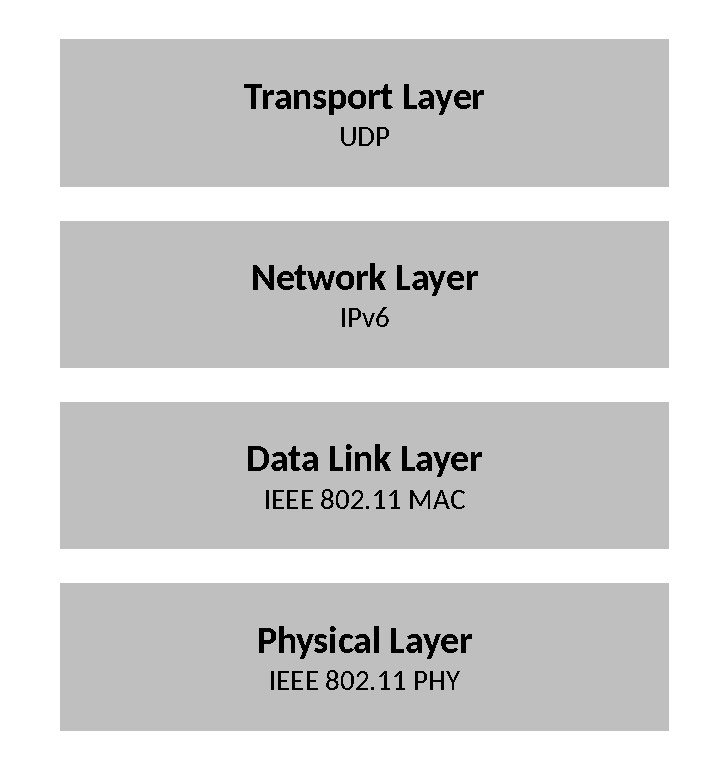
\includegraphics[width=\textwidth/2]{Grafiken-Alex/sensor-osi.pdf}
	\caption{Theoretisch möglicher Aufbau der ersten vier Schichten des \ac{osi}-Modells für einen Sensor}
	\label{sensor-osi}
\end{figure}
Herkömmliche Funkprotokolle - IEEE 802.11 alias Wi-Fi sei hier nur exemplarisch - bedienen die Anforderungen moderner Applikationen. Diese Anforderungen lassen sich zum größten Teil in einem Wort zusammenfassen: Datendurchsatz. Heutige Applikationen für Endanwender benötigen nicht selten Datenraten im Bereich vieler Mbit/s. Diese Geschwindigkeiten werden durch eine hohe Leistungsaufnahme entsprechender Module erkauft. So kann die Leistungsaufnahme eines einfachen Wi-Fi-fähigen \ac{soc} wie des ESP8266EX der Firma Espressif Systems durchaus 500\ac{m}\ac{w} erreichen \cite{esp8266}. Das ist unter Betracht der Tatsache, dass Knopfzellenbatterien für gewöhnlich nicht mehr als 3000mWh Energie speichern ein viel zu hoher Wert. \\
Sensor-Netzwerken benötigen im Gegensatz dazu nur geringe Datenraten, da nur wenige Daten - durchaus im Bereich einiger Bytes - verschickt werden. Andererseits ist hier ganz besonders auf die Leistungsaufnahme zu achten. Um diesen außergewöhnlichen Anforderungen gerecht zu werden, wurde eine Funktechnologie entwickelt und in IEEE 802.15.4 genormt. Weil man bei dieser Technologie auf einen einheitlichen Namen verzichtete - sie wird meist einfach als IEEE 802.15.4 bezeichnet - wird sie in dieser Ausarbeitung 15.4 genannt. \\
Der Standard 15.4 definiert \ac{phy} und \ac{mac} Layer eines Übertragungsprotokolls für \ac{wpan}. Durch lange Ruhephasen wird hier die Leistungsaufnahme einzelner Netzteilnehmer so weit reduziert, dass die gängigen Akkulaufzeiten sich für gewöhnlich im Bereich vieler Monate bewegen. Der Preis dafür ist eine geringe Datenrate von maximal 250 \ac{k}Bit/s bzw. im Sub-1-GHz-Netz sogar nur 40 \ac{k}Bit/s. Was bei anderen Anwendungen inakzeptabel wäre, reicht aber in diesem Falls absolut aus, um einfach Sensordaten ausreichend schnell zu übermitteln. \\
Eine Eigenschaft von \ac{15.4} ist die maximale Paketgröße von 127 Bytes. \ac{ipv6} fordert jedoch eine \ac{mtu} von 1280 Byte. Das bedeutet, dass \ac{mtu} vom auf Layer 2 eingesetzten Protokoll fordert, ein Paket mit maximal 1280 Bytes zu übertragen. Damit ist \ac{15.4} als Übertragungsprotokoll eine IP-Pakets zunächst gar nicht möglich. Darüber hinaus hat der Header des \ac{ipv6}-Protokolls eine Größe von 40 Bytes. Gemeinsam mit dem 8 Byte großen \ac{udp}-Header und dem 25 Byte großen \ac{mac}-Header von \ac{15.4} blieben in einem Paket gerade mal 54 Byte für die Payload, wodurch sich die Datenrate von Nutzdaten auf ca. 17 \ac{k}Bit/s im Sub-1-GHz-Netz reduziert.\cite{grundlagen6lowpan} \\
Diese beiden Hindernisse verlangen von einer Implementierung von \ac{ipv6} auf Basis von \ac{15.4} zwei Eigenschaften:
\begin{itemize}
	\item Fragmentierungs- und Defragmentierungsebene für \ac{ip}-Pakete einführen, um die \ac{mtu} nicht zu verletzen.
	\item Header von \ac{ip} und \ac{udp} möglichst weit komprimieren, um den Anteil an Nutzdaten in einem Datenpaket zu erhöhen.
\end{itemize}
\begin{figure}
	\centering
	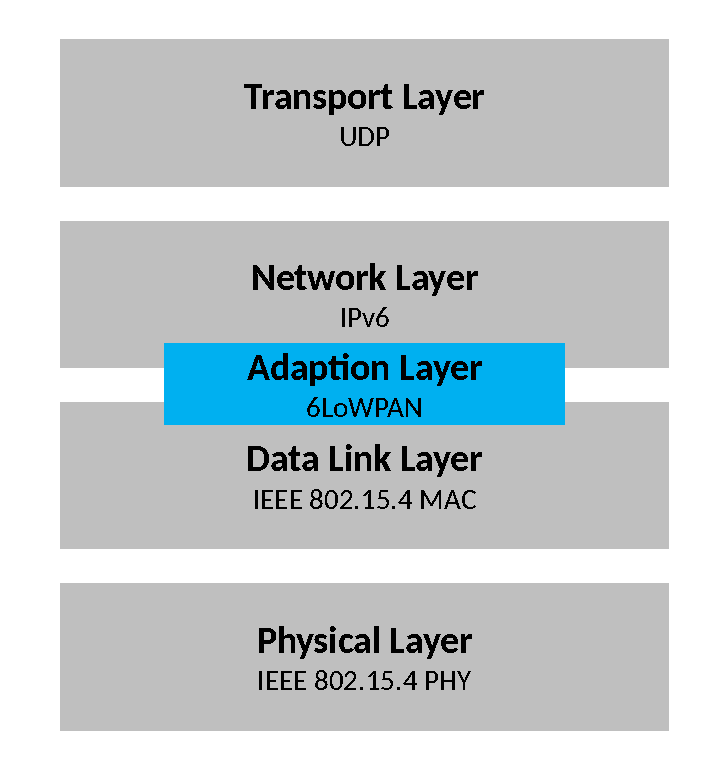
\includegraphics[width=\textwidth/2]{Grafiken-Alex/6lowpan-osi.pdf}
	\caption{Aufbau der ersten vier Schichten des \ac{osi}-Modells unter Verwendung von \ac{6lowpan}}
	\label{6lowpan-osi}
\end{figure}
Um beiden Anforderungen gerecht zu werden, wurde die \ac{6lowpan} Zwischenschicht eingeführt. Diese gliedert sich zwischen Layer 2 (\ac{15.4} \ac{mac}) und Layer 3 (\ac{ipv6}) als Adaptionslayer ein und ermöglicht so die Nutzung von \ac{ip} und darauf aufbauend \ac{udp} auf Basis von \ac{15.4}. Darüber hinaus muss zur Kommunikation nach außen mindestens ein Netzwerkteilnehmer in der Lage sein, Datenpakete, die mit \ac{6lowpan} verschickt wurden in ganz normale UDP/IP-Pakete zu wandeln und über eine herkömmliche Übertragungstechnologie weiterzuleiten. Erst dadurch wird ein einzelner Sensor fähig, am Internet teilzunehmen. Die ersten vier Schichten des OSI-Modells eines solchen Sensors ergeben sich dann also wie in Graphik \ref{6lowpan-osi} gezeigt.